\documentclass[professionalfont]{beamer}

\usepackage{graphicx}
\usepackage{newtxtext,newtxmath}
\usetheme{default}
\usecolortheme{seagull}

\setbeamertemplate{navigation symbols}{}
\setbeamertemplate{itemize item}{\textbullet} 
\setbeamertemplate{title page}{
    \begin{center}
        {\textcolor{blue}{\textbf{\fontsize{12}{14}\selectfont NPHardEval: Dynamic Benchmark on Reasoning Ability of Large Language Models via Complexity Classes}}} \\[1.5cm]
        
        {\fontsize{9}{14}\selectfont Lizhou Fan, et al \\[0.3cm]
        Rutgers University \\[0.3cm]
        February 12, 2024}
    \end{center}
}
% ------------------ Title ------------------

\begin{document}
\frame{\titlepage}


\begin{frame}
\begin{center}
    { \textbf{\textcolor{blue}{ {\fontsize{12}{14}\selectfont Abstract} }} }
\end{center}
\\[0.5cm]

{\fontsize{10}{14}\selectfont 
\begin{itemize}
    \item Current benchmarks are prone to the risk of overfitting
    \item We suggest benchmark with various complexity classes
    
    - P, NP-Complete, NP-Hard
    
    \item Dynamic update to avoid overfitting
    
    - Monthly Update datapoints
\end{itemize}
}

\end{frame}
% ------------------ Slide 1 ------------------

\begin{frame}
\begin{center}
    { \textbf{\textcolor{blue}{ {\fontsize{12}{14}\selectfont Introduction} }} }
\end{center}
\\[0.2cm]

{\fontsize{10}{14}\selectfont 
\begin{itemize}
    \item 3 Complexity classes, 3 Tasks, 100 Problems offered
    
    - Total \( 3\times3\times100=900 \) problems
    
    - {\textcolor{blue}{P}}: Solved in polynomial time
    
    - {\textcolor{blue}{NP-Complete}}: Verified in polynomial time

    - {\textcolor{blue}{NP-Hard}}: No guarantee for polynomial time
\end{itemize}
}

\begin{center}
    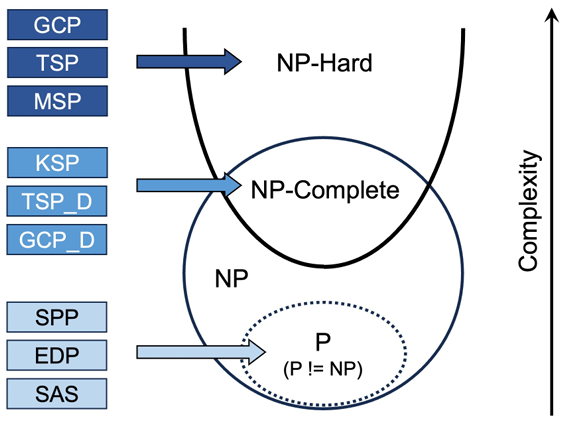
\includegraphics[width=0.6\textwidth]{figure1.png}
\end{center}

\end{frame}
% ------------------ Slide 2 ------------------

\begin{frame}
\begin{center}
    { \textbf{\textcolor{blue}{ {\fontsize{12}{14}\selectfont Introduction} }} }
\end{center}
\\[0.5cm]

{\fontsize{10}{14}\selectfont 
\begin{itemize}
    \item End-to-end automation

    - Generation, Verification are automated by using well-known task

    \item Excluded numerical computation

    - It is noticably difficult for LLMs
    
    - Focusing on pure logical reasoning ability

    \item Difficulty level system

    - For each task, there are 100 problems

    - Each problem has difficulty level from 1 to 10
\end{itemize}
}

\end{frame}
% ------------------ Slide 3 ------------------

\begin{frame}
\begin{center}
    { \textbf{\textcolor{blue}{ {\fontsize{12}{14}\selectfont P Tasks} }} }
\end{center}
\\[0.5cm]

{\fontsize{10}{14}\selectfont 
\begin{itemize}
    \item Sorted Array Search (SAS)
    
    - Finding the position of a target value after sorting a given array

    - Solved by sorting and binary search

    \item Edit Distance Problem (EDP)
    
    - Minimum number of operations to transform one string into another

    - Insertion, deletion, and substitution of a single character.

    - Solved by Dynamic programming

    \item Shortest Path Problem (SPP)
    
    - Finding the shortest path between two nodes in a weighted graph

    - Solved by Dijkstra’s algorithm
\end{itemize}
}

\end{frame}
% ------------------ Slide 4 ------------------

\begin{frame}
\begin{center}
    { \textbf{\textcolor{blue}{ {\fontsize{12}{14}\selectfont NP-Complete Tasks} }} }
\end{center}
\\[0.5cm]

{\fontsize{10}{14}\selectfont 
\begin{itemize}
    \item Traveling Salesman Problem (TSP-D)

    - Can you complete a route, visiting each city at least once?

    - Total travel distance must be less than a specified value

    \item Graph Coloring Problem (GCP-D)

    - Can you color the vertices of a graph using a given number of colors?

    - No two adjacent vertices share the same color

    \item Knapsack Problem (KSP)
    
    - Fill a knapsack of fixed capacity without exceeding it

    - Maximize the total value of the selected items
\end{itemize}
}

\end{frame}
% ------------------ Slide 5 ------------------

\begin{frame}
\begin{center}
    { \textbf{\textcolor{blue}{ {\fontsize{12}{14}\selectfont NP-Hard Tasks} }} }
\end{center}
\\[0.5cm]

{\fontsize{10}{14}\selectfont 
\begin{itemize}
    \item Traveling Salesman Problem (TSP-O)

    - Find the shortest route, visiting each city at least once

    - Important for delivery services, maintenance operations, and sales

    \item Graph Coloring Problem (GCP-O)

    - Color the vertices of a graph with the constraint

    - Used in exam timetabling and register allocation in compilers

    \item Meeting Scheduling Problem (MSP)
    
    - Allocating time slots with participant availability and room capacity

    - Crucial in organizational management for scheduling meetings
\end{itemize}
}

\end{frame}
% ------------------ Slide 6 ------------------

\begin{frame}
\begin{center}
    { \textbf{\textcolor{blue}{ {\fontsize{12}{14}\selectfont Experiment} }} }
\end{center}
\\[0.5cm]

{\fontsize{10}{14}\selectfont 
\begin{itemize}
    \item Model Performance Comparison

    - Compare 5 closed-source models, 7 open-source models

    - Shed light on the relative strengths and weaknesses

    \item Robustness of Benchmark Assessments

    - Examines if the risk of “hacking” the benchmark is prevented

    - Examines if finetuning LLMs on benchmarks leads to overfitting

    \item Generalization through In-context Learning
    
    - Discern whether the model is “learning” or “mimicking”

    - Examine if performance is constant with varing difficulty levels
\end{itemize}
}

\end{frame}
% ------------------ Slide 7 ------------------

\begin{frame}
\begin{center}
    { \textbf{\textcolor{blue}{ {\fontsize{12}{14}\selectfont Result} }} }
\end{center}
\\[0.1cm]

{\fontsize{10}{14}\selectfont 
\begin{itemize}
    \item Increasing difficulty, performance significantly dropped
\end{itemize}
}

\begin{center}
    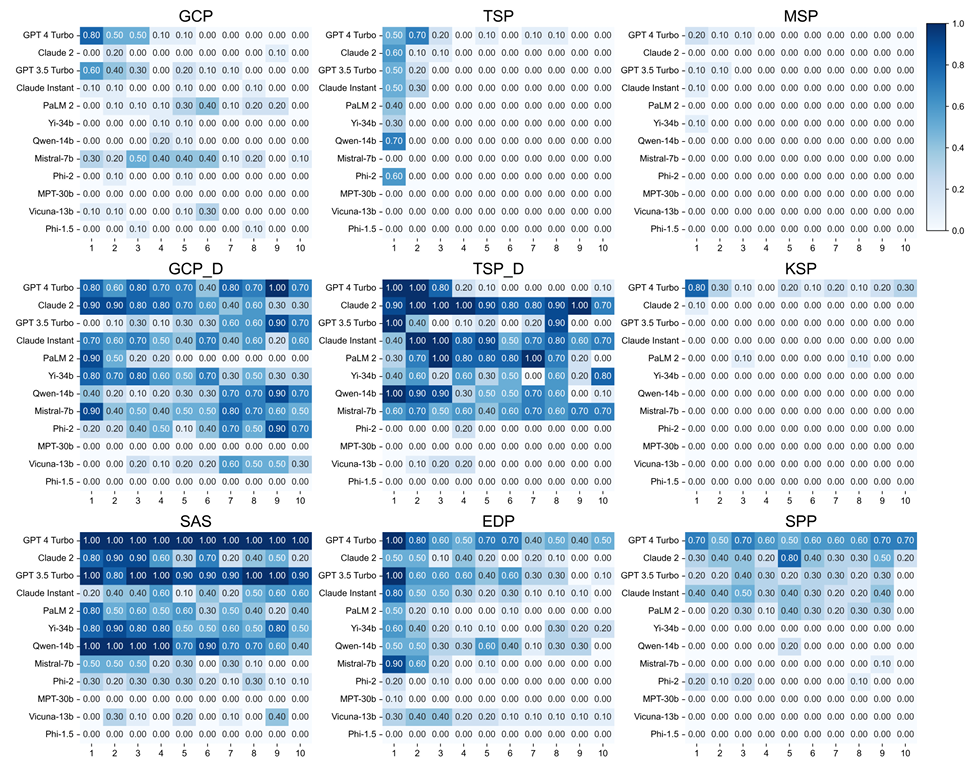
\includegraphics[width=0.9\textwidth]{figure2.png}
\end{center}

\end{frame}
% ------------------ Slide 8 ------------------

\begin{frame}
\begin{center}
    { \textbf{\textcolor{blue}{ {\fontsize{12}{14}\selectfont Limitations} }} }
\end{center}
\\[0.5cm]

{\fontsize{10}{14}\selectfont 
\begin{itemize}
    \item Task Complexity’s Comparison

    - There are only 9 tasks

    - Difficulty is defined as linear increment of variables

    \item Randomness

    - In decision problem, LLMs may find correct answer by luck

    \item Model Update and Emergence

    - Fast-paced evolution of LLMs like Gemini Ultra

    - The analysis based on our benchmark may quickly become outdated
\end{itemize}
}

\end{frame}
% ------------------ Slide 9 ------------------

\end{document}
